\documentclass[11pt,a4paper]{report}

\usepackage[utf8]{inputenc}
\usepackage[T1]{fontenc}
\usepackage[english]{babel}
\usepackage{graphicx}
\usepackage{amsmath} % For \mathbb
\usepackage{amsfonts}
\usepackage{hyperref}
\usepackage{comment}
\usepackage{listings}
%\pagestyle{empty}


%% Numbered exercises
\newcounter{excount}[chapter]
\newenvironment{exercise}[1][]{\addtocounter{excount}{1} \noindent {\bf Question
    \arabic{excount} \ \ #1}\hspace{2mm}}{\vspace{4mm}}


\title{FYS3120 Classical mechanics and electrodynamics\\
Mid-term exam -- Spring term 2019}
\author{}



\begin{document}

\maketitle


\addtocounter{page}{1}


%%%%%%%%%%%%%%%%%%%%
\begin{exercise}{\bf Central potentials\\}
%%%%%%%%%%%%%%%%%%%%
Consider two objects of mass $m_1$ and $m_2$ affected by a time-independent central potential $V(r)$ in regular three-dimensional space, where $\vec r$ gives the distance between the objects $\vec r = \vec r_1- \vec r_2$.

\begin{itemize}
\item[{\bf a)}] Find the number of degrees of freedom, and identify appropriate generalized coordinates. [1 point] \par 
%%%%%%%%%%%%%%%%%%%%% 1.a
The number of degrees of freedom, $d$ is a function of the number of bodies, $N$ and the number of constraint functions, $M$, on the system.
The system consists of two bodies, $N=2$, and no constraints, $M=0$. Which means that $d=3N-M=6$. \par 
The components of $\vec{r}=\vec{r}_1-\vec{r}_2$ and $\vec{R}=\frac{\mu}{m_2}\vec{r}_1+\frac{\mu}{m_1}\vec{r}_2$, where $\mu=\frac{m_1m_2}{m_1+m_2}$, are chosen as the generalized coordinates.

\item[{\bf b)}] Explain why the motion of three of the generalized coordinates can be solved trivially, and write down the solution. [1 point] \par 


%%%%%%%%%%%%%%%%%%%%% 1.b 
Using the results from assignment 4 (see appendix at the end of this document), the Lagrangian of this two body system may be expressed in terms of $\vec{r}$ and $\vec{R}$ as:
\begin{equation}
L=\frac{1}{2}(m_1+m_2)\dot{R}^2 +\frac{1}{2} \mu \dot{r}^2 -V(\vec{r})
\end{equation}
Finding the Lagrange's equations:
\begin{align}
\frac{d}{dt} \frac{\partial L}{\partial \dot{q_i}}-\frac{\partial L}{\partial q_i}=0 \\
\frac{d}{dt} \frac{\partial L}{\partial \dot{R_i}}-\frac{\partial L}{\partial R_i}=(m_1+m_2)\ddot{R}_i=0 \label{eq.1.b.ddotR}\\
\frac{d}{dt} \frac{\partial L}{\partial \dot{r_i}}-\frac{\partial L}{\partial r_i}=\mu \ddot{r_i}-\frac{\partial V}{\partial r_i}=0 \implies \mu\ddot{r}_i=\frac{\partial V}{\partial r_i}
\end{align}

\eqref{eq.1.b.ddotR} shows that the center of mass moves at a constant speed, and it may therefore be chosen as an inertial reference frame. This means that $\vec{R}=(0,0,0)$ and $\dot{R_i}=0$. Thus the Lagrangian reduces to $L=\frac{1}{2}\mu \dot{\vec{r}}^2-V(r)$.

\item[{\bf c)}] Explain why the angular momentum of the reduced mass $\mu$,
\begin{equation}
\vec\ell = \vec r \times \vec p= \vec r \times \mu\dot{\vec r},
\end{equation}
where
\begin{equation}
\mu= \frac{m_1m_2}{m_1+m_2},
\end{equation}
is a constant of motion.
[1 point] \par 
%%%%%%%%%%%%%%%%%%%% 1.c const of motion p.41
As no outside forces are working on the system, the torque $\tau=\frac{d \vec{\ell}}{dt}=0$, which shows that $\vec{\ell}$ is independent of time, which also means that it is a constant of motion.


\item[{\bf d)}] Explain why this leads to the motion being confined to the plane perpendicular to $\vec\ell$. [1 point]

%%%%%%%%%%%%%%%%%%% 1.d
The vector $\vec{c}=\vec{a} \times \vec{b}$ is by the definition of the cross product parallel to the plane containing $\vec{a}$ and $\vec{b}$. As $\vec\ell = \vec r \times \vec p$, and $\vec \ell$ is conserved, the plane containing $\vec{r}$ and $\vec{p}$ is constant, which mean that the motion is confined to a plane perpendicular to $\vec{\ell}$.



\item[{\bf e)}] Choosing $\vec\ell= \ell\hat k$, {\it i.e.}\ that the angular momentum is in the $z$-direction, we can switch to the polar coordinates $(r,\phi)$, where $\phi$ is the angle in the $xy$-plane. Show that the equations of motion for these coordinates are
\begin{equation}
\mu\ddot r-\frac{\ell^2}{\mu r^3}+\frac{\partial V}{\partial r}=0,\label{eq:LEQ_r}
\end{equation}
and
\begin{equation}
\dot\phi=\frac{\ell}{\mu r^2}\label{eq:LEQ_phi}.
\end{equation}
[3 points] \par


%%%%%%%%%%%%%%%%%%%%%% 1.e
As the motion is confined to a plane, polar coordinates may be used to be used to describe the system, with general coordinates $r, \phi$, such that $\vec{r}=r \vec{e_r}+\phi \vec{e_\phi}$, which means that $\dot{\vec{r}}=\dot{r} \vec{e_r}+ r \dot{\phi} \vec{e_\phi}$. This yields the Lagrangian:
\begin{align}
L=\frac{1}{2}\mu (\dot{r}^2+r^2\dot{\phi}^2)-V(r) \label{eq:1.e.L}
\end{align} 

Lagrange's equations in polar coordinates:
\begin{align}
&\frac{d}{dt}\frac{\partial L}{\partial \dot{\phi}}-\frac{\partial L}{\partial \phi}=\mu r^2 \ddot{\phi}=0 \\
&\frac{d}{dt}\frac{\partial L}{\partial \dot{r}}-\frac{\partial L}{\partial r}=\frac{d}{dt}(\mu\dot{r})-(\mu r \dot{\phi}^2-\frac{\partial V}{\partial r})=\mu\ddot{r}-\mu r \dot{\phi}^2+\frac{\partial V}{\partial r} \label{eq:1.e.dr}
\end{align} 

\begin{align}
\eqref{eq:1.e.dr}=\mu\ddot{r}-\mu r \frac{\ell^2}{\mu^2 r^4}+\frac{\partial V}{\partial r}=\mu\ddot{r}-\frac{\ell^2}{\mu r^3}+\frac{\partial V}{\partial r}=0
\end{align} 

As $\frac{\partial L}{\partial \phi}=0$, $\phi$ is a cyclic coordinate. Thus the conjugate momentum, $p_i=\frac{\partial L}{\partial  \dot{q}_i}$ for $\phi$ is
\begin{equation}
p_{\phi}=\frac{\partial L}{\partial \dot{\phi}}=\mu r^2 \dot{\phi}
\end{equation}
which is a constant of motion corresponding to $\ell$, so $\dot{\phi}=\frac{\ell}{\mu r^2}$

\item[{\bf f)}] Find the corresponding Hamiltonian in terms of the generalized coordinates $(r,\phi)$ and generalized momenta $(p_r,p_\phi)$, and write down Hamilton's equations for this system.  [3 points] \par 



%%%%%%%%%%%%%%%%%%%% 1.f
Finding the generalized momenta: 
\begin{align}
p_i=\frac{\partial L}{\partial \dot{q_i}} \\
p_r=\frac{\partial L}{\partial \dot{r}}=\frac{\partial}{\partial t}\frac{1}{2}\mu (\dot{r}^2+r^2\dot{\phi}^2)-V(r) = \mu \dot{r}\\
\end{align}
From 1.e), $p_{\phi}=\mu r^2 \dot{\phi}$ \par 
The definition of the Hamiltonian is:
\begin{align*}
H=\sum_i p_i \dot{q_i}-L
\end{align*}
So,
\begin{align}
H&= p_{\phi} \dot{\phi} + p_r\dot{r}-(\frac{1}{2}\mu (\dot{r}^2+r^2\dot{\phi}^2)-V(r))\\
&= p_{\phi} \dot{\phi} + p_r\dot{r}-\frac{1}{2} p_r \dot{r} -\frac{1}{2}p_\phi \dot{\phi}   +V(r) \\
&= \frac{1}{2} p_r \dot{r} +\frac{1}{2}p_\phi \dot{\phi}   +V(r)\\
&=  \frac{1}{2} \frac{p_r^2}{\mu}  +\frac{1}{2}\frac{p_\phi^2}{\mu r^2}    +V(r) \label{eq:H1}
\end{align}
The Hamilton's equations are
\begin{align*}
\dot{q_i}=\frac{\partial H}{\partial p_i} \\
\dot{p_i}=-\frac{\partial H}{\partial q_i} \\
\end{align*}
So 
\begin{align}
&\dot{r}=\frac{\partial H}{\partial p_r}=\frac{p_r}{\mu}=\dot{r} \\
&\dot{p_r}=-\frac{\partial H}{\partial r}=\frac{p_\phi^2}{\mu r^3}-\frac{\partial V}{\partial r} \\
&\dot{\phi}=\frac{\partial H}{\partial p_\phi} =\frac{p_\phi}{\mu r^2}\\
&\dot{p_\phi}=-\frac{\partial H}{\partial \phi}=0 
\end{align}
\item[{\bf g)}] Explain why the Hamiltonian $H$ of this system is a constant of motion and what the physical interpretation of $H$ is. [1 point] \par 

As there is no explicit time dependency in the Hamiltonian in 1.f), the Hamiltonian has no time dependency: $\frac{dH}{dt}=\frac{\partial H}{\partial t}=0$, and is thus a constant of motion. The physical interpretation of $H$ is the total energy of the system; $E_{tot}=K+V$.
\end{itemize}
\end{exercise}


%%%%%%%%%%%%%%%%%%%%
\begin{exercise}{\bf Orbital motion\\}
%%%%%%%%%%%%%%%%%%%%
Consider the gravitational potential between two objects of mass $m_1$ and $m_2$,
\begin{equation}
V(r)=-\frac{Gm_1m_2}{r},\label{eq:grav_pot}
\end{equation}
where $G$ is Newton's gravitational constant.
\begin{itemize}
\item[{\bf a)}] Find Hamilton's equations for this system. [1 point] \par

%%%%%%%%%% 2.a
A gravitational potential is a central potential, as such, $H$ from question 1 may used \eqref{eq:H1}, and the correct $V(r)$ applied:
\begin{align}
H &=  \frac{1}{2} \frac{p_r^2}{\mu}  +\frac{1}{2}\frac{p_\phi^2}{\mu r^2}  -\frac{Gm_1m_2}{r}
\label{eq:2.a.H}
\end{align}
Where $\mu=\frac{m_1m_2}{m_1+m_2}$, $p_r=\mu \dot{r}$ and $p_\phi=\mu r^2 \dot{\phi}=\ell$
 \item[{\bf b)}] Make a two-dimensional plot of the phase space for the distance $r$ between the objects, and its generalized momentum $p_r$, for concreteness fixing the masses to be those of the International Space Station (ISS) orbiting the Earth, varying $\ell$.

Give a qualitative description of the different types of motion that can be read out of the diagram and comment on how the situation changes with increasing $\ell$. {\it Hint:} For those using {\tt python} the plotting framework {\tt pyplot} has a useful plotting command for phase space plots called {\tt streamplot}.  [4 points] \par 

Using the code from the code section of the appendix, the phase space of the two body system consisting of the Earth ($m_1=5.972e24$ kg) and the ISS ($m_2=419725$kg) is shown as a function $\ell$  in figure \ref{fig:phase}, for four selected values of $\ell$ found through trial and error. \par 

Trajectories in phase space diagrams have conserved energy, such that each trajectory represents one solution (initial position and velocity) to the two body problem. The diagrams in figure \ref{fig:phase} show several such trajectories. One type of these trajectories present in all four diagrams is the vertical line, going from negative momentum to positive momentum. These lines represent the ISS shooting towards the Earth with high velocity, then going past the Earth in such a short time that that the radial velocity component hardly changes. \par

 In the upper left corner, the angular momentum is relatively low compared to the diagrams, resulting in phase space trajectories that are mostly associated with the ISS either moving at increasing velocity towards the earth (trajectories pointing towards lower values of $r$) - and possibly entering the atmosphere (these trajectories would disappear down towards  large negative $p_r$), or away from the Earth with decreasing velocities (trajectories pointing towards increasing values of $r$)-possibly escaping the Earth's gravitational pull. In the case of the trajectories which change the sign of $p_r$, the ISS initially moving away from the Earth, and is at $p_r=0$ completely de-accelerated by the gravitational force, and pulled back towards the Earth. \par 

In the upper right diagram of figure \ref{fig:phase} $\ell$ is close to a critical value at which some solutions produce elliptical orbits for the ISS around the Earth. Such trajectories are identified by going from negative values of $p_r$, to positive values of $p_r$ at a minimum value of $r$ (perihelion), before gradually decreasing in $p_r$ while increasing in $r$. Then, at a maxima of $r$ (aphelion), the ISS is de-accelerated and begins the part of it's orbit where it is heading "towards" Earth again.\par

In the lower left diagram, the angular momentum is higher than in the upper right, such that most of the trajectories shown are hyperbolic - which corresponds to a hyperbolic motion of the ISS, going towards the earth, then being slingshot out of proximity again. The same goes for the bottom right diagram, only with even larger hyperbolic motion.\par 

To conclude, as $\ell$ increases, the ISS goes from either escaping or possibly crashing into the atmosphere (depending on initial conditions), to - for certain initial conditions - maintaining a stable orbit. As $\ell$ increases further, these orbits have increasing radii, to the point where the ISS has a hyperbolic motion.
\begin{figure}[!htb]
        \centering 
         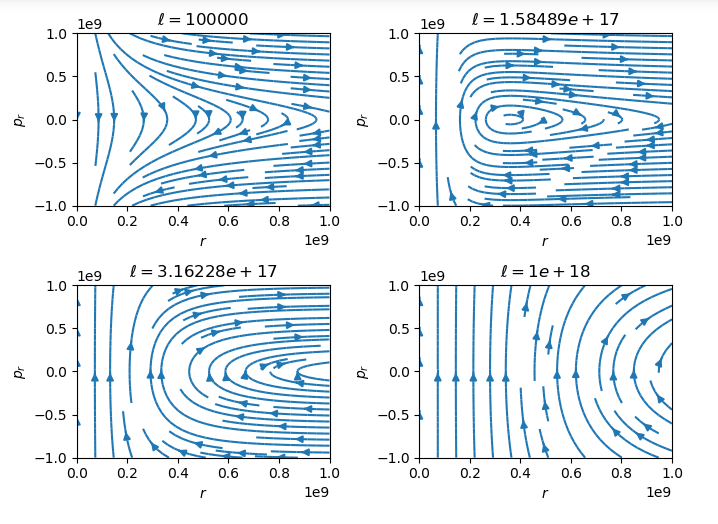
\includegraphics[scale=.7]{phases.png} 
        \caption{Phase space plot for the Earth and the ISS -question 2.b)}
        \label{fig:phase}   
\end{figure}  



\item[{\bf c)}] Use the Lagrange equations to show that the differential equation for the orbit equation $r(\phi)$, where $\phi$ is the polar angle of the motion, is
\begin{equation}
\frac{d^2r}{d\phi^2}-\frac{2}{ r}\left(\frac{dr}{d\phi}\right)^2-r+\frac{Gm_1m_2\mu }{\ell^2}r^2=0. \label{eq:2c.diffeq}
\end{equation}
[2 points] \par 

%%%%%%%%%%%%%%% 2.c

Using the Lagrangian equations from question 1 with the potential $V(r)=-\frac{Gm_1m_2}{r}$, and the time derivative of $\dot{\phi}$
\begin{equation*}
\frac{d \dot{\phi}}{dt}= \frac{d}{dt} \frac{\ell}{\mu r^2}=-2\frac{\ell}{\mu r^3}\frac{dr}{dt}=-2\frac{\ell}{\mu r^3}\frac{dr}{d\phi}\frac{d\phi}{dt}=-2 \frac{\dot{\phi}^2}{r} \frac{dr}{d\phi}
\end{equation*}
gives:
\begin{align*}
&\mu\ddot r-\frac{\ell^2}{\mu r^3}+\frac{\partial V}{\partial r}=0\\
&\mu \frac{d}{dt}\frac{d}{dt} r-\frac{\ell^2}{\mu r^3}-\frac{\partial }{\partial r}\frac{Gm_1m_2}{r} =0\\
&\mu \frac{d}{dt}\left(\frac{dr}{d\phi}\frac{d \phi}{dt}\right) -\frac{\ell^2}{\mu r}+\frac{Gm_1m_2}{r^2} =0\\
&\mu \frac{d}{dt}\left(\frac{dr}{d\phi}\dot{\phi} \right) -\frac{\ell^2}{\mu r^3}+\frac{Gm_1m_2}{r^2} =0\\
&\mu \dot{\phi}\frac{d}{dt}(\frac{dr}{d\phi}) + \mu \frac{dr}{d\phi} \frac{d \dot{\phi}}{dt} -\frac{\ell^2}{\mu r^3}+\frac{Gm_1m_2}{r^2} =0\\
&\mu \dot{\phi}\frac{d\phi}{dt} \frac{d}{d\phi}(\frac{dr}{d\phi}) -2 \mu \frac{\dot{\phi}^2}{r} \left(\frac{dr}{d\phi}\right)^2  \  -\frac{\ell^2}{\mu r^3}+\frac{Gm_1m_2}{r^2} =0\\
&\mu \dot{\phi}^2 \frac{d^2r}{d\phi^2} -2 \mu \frac{\dot{\phi}^2}{r} \left(\frac{dr}{d\phi}\right)^2  \  -\frac{\ell^2}{\mu r^3}+\frac{Gm_1m_2}{r^2} =0\\
&\frac{d^2r}{d\phi^2} - \frac{2}{r} \left(\frac{dr}{d\phi}\right)^2  \  - \frac{1}{\mu}\frac{\mu^2 r^4}{ \ell^2} \frac{\ell^2}{\mu r^3}+\frac{1}{\mu}\frac{\mu^2 r^4}{ \ell^2}\frac{Gm_1m_2}{r^2} =0\\
&\frac{d^2r}{d\phi^2} - \frac{2}{r} \left(\frac{dr}{d\phi}\right)^2  \  - r+\frac{Gm_1m_2 \mu}{\ell^2} r^2=0\\
\end{align*}



\item[{\bf d)}] Show that complete set of solutions for the orbit equation  is
\begin{equation}
r(\phi)= \frac{r_0}{1-\varepsilon \cos(\phi-\phi_0)},
\end{equation}
where $\varepsilon$ is called the {\bf eccentricity} and $\phi_0$ the {\bf phase}. Find $r_0$.
{\it Hint:} The substitution $s=1/r$ is very useful. [2 points] \par

%%%%%%%%%%%%%%%%%%% 2.d 
Using $s=1/r$,
\begin{equation}
\frac{ds}{d\phi}=\frac{ds}{dr}\frac{dr}{d\phi}=\frac{d}{dr}\left(\frac{1}{r}\right)\frac{dr}{d\phi}=-\frac{1}{r^2}\frac{dr}{d\phi} \implies \frac{dr}{d\phi}=-\frac{1}{s^2}\frac{ds}{d\phi}
\end{equation}
Substituting into \eqref{eq:2c.diffeq}: 
\begin{align}
&\frac{d^2r}{d\phi^2}-\frac{2}{ r}\left(\frac{dr}{d\phi}\right)^2-r+\frac{Gm_1m_2\mu }{\ell^2}r^2=0\\
	&\frac{d}{d\phi}\left(-\frac{1}{s^2}\frac{ds}{d\phi}\right) -2s\left(-\frac{1}{s^2}\frac{ds}{d\phi} \right)^2-\frac{1}{s}+\frac{Gm_1m_2\mu }{\ell^2 s^2}=0 \\
	&-\frac{d}{d\phi}\left(\frac{1}{s^2}\right)\frac{ds}{d\phi}-\frac{d}{d\phi}\left(\frac{ds}{d\phi}\right)\frac{1}{s^2} -\frac{2}{s^3}\left(\frac{ds}{d\phi} \right)^2-\frac{1}{s}+\frac{Gm_1m_2\mu }{\ell^2 s^2}=0 \\
	&\frac{2}{s^3} \frac{ds}{d\phi}\frac{ds}{d\phi}-\frac{1}{s^2}\frac{d^2s}{d\phi} -\frac{2}{s^3}\left(\frac{ds}{d\phi} \right)^2-\frac{1}{s}+\frac{Gm_1m_2\mu }{\ell^2 s^2}=0 \\
		&-\frac{1}{s^2}\frac{d^2s}{d\phi} -\frac{1}{s}+\frac{Gm_1m_2\mu }{\ell^2 s^2}=0 \\		
	&\implies 	\frac{1}{s^2}\frac{d^2s}{d\phi} +\frac{1}{s}=\frac{Gm_1m_2\mu }{\ell^2 s^2}\\
	&\implies \frac{d^2s}{d\phi} + s=\frac{Gm_1m_2\mu }{\ell^2 }
\end{align}

which is a nonhomogeneous second order differential equation. 
The general solution to the homogeneous equation (harmonic oscillator equation): 
\begin{equation}
\frac{d^2s}{d\phi} + s=0
\end{equation}  is $s_1= A \cos(\phi-\phi_0)$, where $A$ is a constant, and $\phi_0$ the phase. \par 
A solution to the nonhomegenous equation is the constant solution: $s_0=\frac{Gm_1m_2\mu }{\ell^2 }$. Thus the solution  of the differential equation may be written as: 
\begin{equation}
s(\phi)=
\frac{Gm_1m_2\mu }{\ell^2 }+A \cos(\phi-\phi_0)=\frac{Gm_1m_2\mu }{\ell^2 }\left(1+\varepsilon \cos(\phi-\phi_0)\right)
\end{equation} \par 
The choice of $A$ and $\phi_0$ correspond to particular instances of the problem, such that $A$ may be written as $-A$, thus: 
\begin{equation}
s(\phi)=\frac{Gm_1m_2\mu }{\ell^2 }\left(1-\varepsilon \cos(\phi-\phi_0)\right)
\end{equation} 
Where $\epsilon=\frac{A l^2}{Gm_1m_2\mu}$ \par 
Solving for $r(\phi)$ by substituting in $r=\frac{1}{s}$ and rearranging:
\begin{align*}
r(\phi)=\frac{\frac{\ell^2 }{Gm_1m_2\mu}}{1-\varepsilon \cos(\phi-\phi_0)}=\frac{r_0}{1-\varepsilon \cos(\phi-\phi_0)}
\end{align*} 
As shown above, $r_0=\frac{\ell^2 }{Gm_1m_2\mu}$, where $\ell$ is a constant of motion corresponding to a specific orbit.

\item[{\bf e)}] Find an expression for the total energy in terms of the eccentricity $\varepsilon$. [2 points] \par 

\begin{align*}
\dot{r}(\phi)&=\frac{d}{dt}\frac{r_0}{(1-\varepsilon \cos(\phi-\phi_0)}=-\frac{r_0(\varepsilon sin(\phi-\phi_0)}{(1-\varepsilon \cos(\phi-\phi_0)^2}\frac{d\phi}{dt}=-\frac{r_0(\varepsilon sin(\phi-\phi_0)}{(1-\varepsilon \cos(\phi-\phi_0)^2}\frac{\ell}{\mu (r(\phi))^2}\\
&=-\frac{r_0(\varepsilon sin(\phi-\phi_0)}{(1-\varepsilon \cos(\phi-\phi_0)^2}\frac{\ell}{\mu r_0^2}(1-\varepsilon \cos(\phi-\phi_0)^2\\
&=-\frac{\varepsilon \ell}{\mu r_0}\sin(\phi-\phi_0)
\end{align*}

As $\frac{dH}{dt}=\frac{dE_{tot}}{dt}=0$, finding the total energy, $E_{tot}$, may be done at an arbitrary angle $\phi$. Using  \eqref{eq:2.a.H} and substituting  $p_r=\mu \dot{r}(\phi)$ and $p_\phi=\ell$, yields $H=\frac{1}{2}\mu(\dot{r}(\phi))^2+\frac{1}{2}\frac{\ell^2}{\mu (r(\phi))^2}-\frac{Gm_1m_2}{r}=E_{tot}$, may therefore be calculated at $\phi=\phi_0$, where  $r(\phi_0)=\frac{\ell^2}{\eta \mu(1-\varepsilon)}$ , where $\nu=Gm_1m_2$, and $\dot{r}(\phi_0)=-\frac{\varepsilon \ell}{\mu r_0}\sin(\phi_0-\phi_0)=0$. So;
\begin{align*}
	H&=\frac{1}{2}\frac{\ell^2}{\mu (r(\phi_0))^2}-\frac{Gm_1m_2}{r(\phi)} \\
	&=\frac{1}{2}\frac{\eta^2\mu(1-\varepsilon)^2}{\ell^2}-\frac{\eta^2 \mu(1-\varepsilon)}{\ell^2}=\frac{\eta^2 \mu}{\ell^2}\left(\frac{(1-\varepsilon)^2}{2}-1+\varepsilon\right)=\frac{\eta^2 \mu}{\ell^2}(\frac{\varepsilon^2}{2}-\frac{1}{2})\\
	&=\frac{G^2m_1^2m_2^2 \mu}{2\ell}(\varepsilon^2-1)
\end{align*}
Which means that $E_{tot}(\varepsilon)=\frac{Gm_1m_2}{2r_0}(\epsilon^2-1)$



\item[{\bf f)}] If an astronaut jumped off the ISS directly towards Earth, what would happen to her orbit? Assume, for simplicity, that the ISS is in a circular orbit. [2 points] \par

The total energy of the astronaut right after the jump is $E_{tot}=-\frac{G^2m_1m_2}{2\ell}+\frac{1}{2} \mu \dot{\vec{r}}^2$, where $E(\epsilon=0)$ is the energy associated with being the same orbit as the ISS, and the second term being the additional kinetic energy from the jump. 

\begin{align*}
E_{tot}=-\frac{G^2 m_1^2m_2^2 \mu}{2 \ell^2}+\frac{1}{2}\mu \dot{\vec{r}}^2
\end{align*}
Where $m_1$ is the mass of the Earth, and $m_2$ is the mass of the astronaut. $\ell=r\mu\dot{r}=r_{ISS}\mu v_{ISS}$, where $v_{ISS}$ is the tangential velocity of the ISS, and $r_{ISS}$ the radius of the orbit of the ISS. Using that $E_{tot}=E_{tot}(\varepsilon')$, the eccentricity of the astronaut's new orbit, $\varepsilon'$ may be found. Due to the fact that the astronaut is jumping towards the earth, the angular momentum is preserved.
\begin{align*}
-\frac{G^2 m_1^2m_2^2 \mu}{2 \ell^2}+\frac{1}{2}\mu \dot{\vec{r}}^2=\frac{G^2m_1^2m_2^2 \mu}{2\ell^2}(\varepsilon'^2-1)\\
\frac{G^2m_1^2m_2^2 \mu}{2\ell^2}(\varepsilon'^2-1+1)=\frac{1}{2}\mu \dot{r}^2 \\
\varepsilon'^2=\frac{\dot{r}^2 \ell^2}{G^2 m_1^2 m_2^2}\\
\varepsilon'=\frac{\dot{r}\mu r_{ISS} v_{iss}}{Gm_1m_2}
\end{align*}
Using the mass of the Earth and and assuming that an astronaut with complementary rig ways around $100$ kg and a jump performed within reasonable limits of human physicality, the new eccentricity is $\approx 0$ (Deadline is closing in, and I cannot find my exact calculations among my notes, although I remember the answer). Thus the astronaut starts orbiting the Earth in a lonely orbit that is slightly more elliptic than the ISS, but still almost circular. In reality she would perhaps start orbiting around the ISS - although I am not entirely certain of this. If she wanted to enter atmosphere, she should have had to have jumped in the opposite direction of the ISS's tangential velocity using some advanced performance enchanting utilities - the required speed is quite high.
\end{itemize}
\end{exercise}



\section*{Appendix}
\subsection*{Excerpt from assignment 4}
\textit{Excerpt from my solution to problem 2. in assignment 4, showing that $L=K-V=\frac{1}{2}m_1 \dot{\vec{r_1}}^2+\frac{1}{2}m_2\dot{\vec{r_2}}^2-V(\vec{r}_1-\vec{r}_2)$ may be expressed in terms of $\vec{r}$ and $\vec{R}$ as shown in \eqref{eq:app.2}:}
\begin{itemize}
\item[\bf b)] Make the change of variables to the coordinates $(\vec r, \vec R)$, where
\begin{eqnarray}
{\vec r} &=& {\vec r}_1 -{\vec r}_2,\\
{\vec R} &=& \frac{m_1}{m_1+ m_2}{\vec r}_1 + \frac{m_2}{m_1+ m_2}{\vec r}_2, 
\label{eq:2b}
\end{eqnarray}
and show that the resulting Lagrangian is
\begin{equation}
L= \frac{1}{2}(m_1+m_2)\dot{\vec R}^2+ \frac{1}{2}\mu\dot{\vec r}^2-V(r),\label{eq:app.2}
\end{equation}
where
\begin{equation}
\mu=\frac{m_1m_2}{m_1+ m_2},
\end{equation}
is the {\bf reduced mass}.

\item (\ref{eq:2b}) yields $\vec{r}_1=\alpha_2\vec{r}+\vec{R}, \vec{r}_2=-\alpha_1\vec{r}+\vec{R}$, and $\vec{\dot{r}}_1=\alpha_2\dot{\vec{r}}+\dot{\vec{R}}, \vec{\dot{r}}_2=-\alpha_1\dot{\vec{r}}+\dot{\vec{R}}$,  where 
$\alpha_1=\frac{m_1}{m_1+m2}, \alpha_2= \frac{m_2}{m_1+m2}$. Inserting these expressions into the Lagrangian: 
\item \begin{align*}
L=\frac{1}{2}m_1 (\alpha_2\dot{\vec{r}}+\dot{\vec{R}})^2+\frac{1}{2}m_2 (-\alpha_1\dot{\vec{r}}+\dot{\vec{R}})^2 -V(\vec{r}) \\
=\frac{1}{2}m_1 (\alpha_2^2 \dot{r}^2+\alpha_2\dot{\vec{r}}\dot{\vec{R}}+\dot{R}^2)+\frac{1}{2}m_2 (\alpha_1^2\dot{r}^2-\alpha_1\dot{\vec{r}}\dot{\vec{R}}+\dot{R}) -V(\vec{r})\\
=\frac{1}{2}m_1 (\alpha_2^2 \dot{r}^2+\dot{R}^2)+\frac{1}{2}m_2 (\alpha_1^2\dot{r}^2+\dot{R})^2 -V(\vec{r})\\
=\frac{1}{2}(m_1+m_2)\dot{R}^2 +\frac{1}{2}m_1\alpha_2^2 \dot{r}^2+\frac{1}{2}m_2 \alpha_1^2\dot{r}^2 -V(\vec{r})\\
=\frac{1}{2}(m_1+m_2)\dot{R}^2 +(\alpha_2+\alpha_1)\frac{1}{2} \mu \dot{r}^2 -V(\vec{r})\\
=\frac{1}{2}(m_1+m_2)\dot{R}^2 +\frac{1}{2} \mu \dot{r}^2 -V(\vec{r})
\end{align*}
\end{itemize}
\subsection*{Code}
Below is the python 3.0 code used to produce the phase space plot in 2.b)
\begin{lstlisting}
import numpy as np
%matplotlib notebook
import matplotlib.pyplot as plt
import matplotlib.gridspec as gridspec

m1=5.972e24 #mass of earth in kgs
m2=419725 #mass of ISS in kgs
mu=m1*m2/(m1+m2)
G=6.67408e-11

r=np.linspace(1e3,1e9)
p=np.linspace(-1e9,1e9)
L=np.array([10**5,10**17.2,10**17.5,10**18])
import numpy as np
import matplotlib.pyplot as plt
import matplotlib.gridspec as gridspec

fig = plt.figure(figsize=(7, 9))
gs = gridspec.GridSpec(nrows=3, ncols=2, height_ratios=[1, 1, 2])

R,P = np.meshgrid(r, p)
for i in range(len(L)):
    U = P/mu
    V = (L[i]**2)/(mu*R**3)-G*m1*m2/R**2

    #  Varying density along a streamline
    ax0 = fig.add_subplot(gs[i//2, i%2])
    ax0.streamplot(R, P, U, V, density=[0.5, 1])
    ax0.set_title("$\ell=%g$"%(L[i]))
    ax0.set_xlabel('$r$')
    ax0.set_ylabel('$p_r$')
  
plt.tight_layout()
plt.show()
\end{lstlisting}



\end{document}